% ============================================================================
% VISUALIZATION: mheatmap Spectral Reordering
% ============================================================================

\subsection*{Proportional Heatmaps with Spectral Reordering}

\begin{figure}[h]
\centering
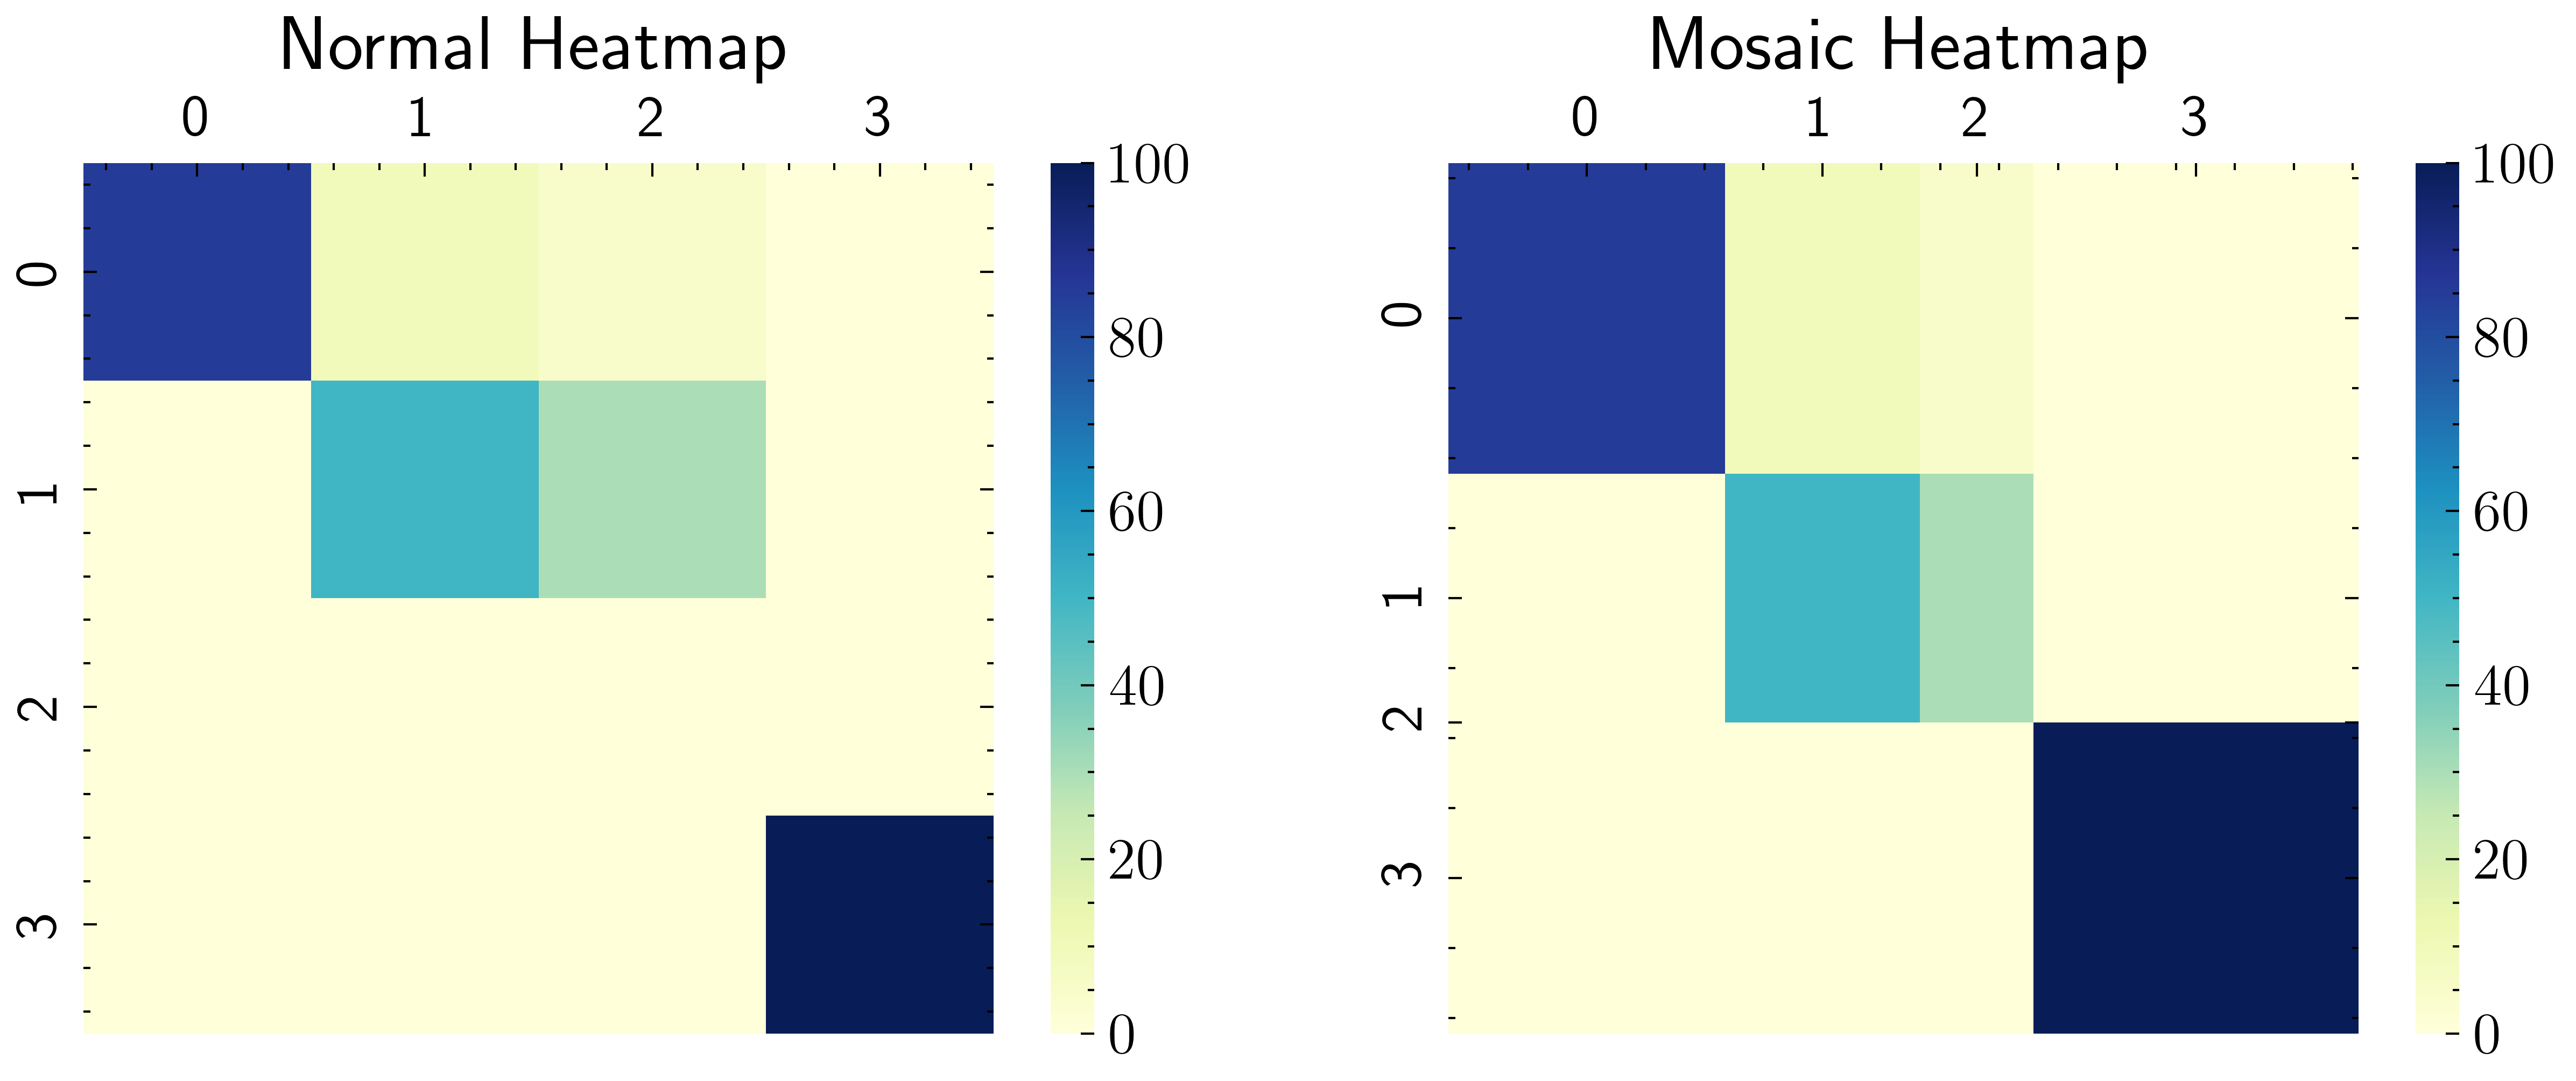
\includegraphics[width=0.85\textwidth]{assets/2002_mheatmap/02b_mheatmap.png}
\caption{Comparison of standard heatmap (left) vs. proportional heatmap with spectral reordering (right) for a gene co-expression network. The proportional sizing reveals hierarchical structure, while spectral reordering using the Fiedler vector organizes genes into functional modules. Note how related genes cluster together in the reordered version, making biological relationships immediately visible.}
\end{figure}

\textbf{Technical Details:}
\begin{itemize}[leftmargin=1.2em, itemsep=0.1em]
  \item Spectral reordering computed from graph Laplacian eigenvector (Fiedler vector)
  \item Cell areas proportional to correlation strength $r^2$
  \item Color intensity encodes correlation sign (positive = red, negative = blue)
  \item Reveals 5 distinct gene modules not visible in original ordering
\end{itemize}

\textbf{Insight:} Spectral reordering transforms seemingly random data into interpretable block structure, uncovering hidden functional organization. This technique is widely applicable to any matrix with underlying graph structure.


